%%%%% Magnetisches Feld %%%%%
%%  %%


%Some sample text to be displayed above the first subsection

%\subsection{Prinzip}

%Ein Zyklotron besteht aus Zwei hohlen, halbzylindrischen und Duanden an denen eine Spannung mit unterschiedlichem Vorzeichen anliegt, und darüber bzw. darunter liegende Magneten, die ein homogenes Magnetfeld erzeugen. Zudem gibt es einen Einlass und einen Auslass für Teilchen.

%\begin{wrapfigure}{r}{0.4\textwidth} \label{Zyklo}
%
%	\vspace{-10pt}
%	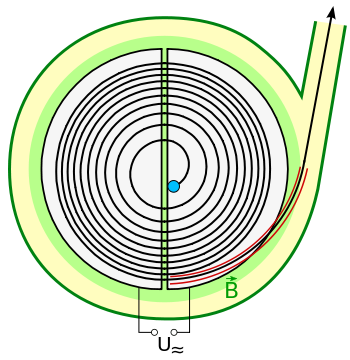
\includegraphics[width=0.35\textwidth]{Zyklotron_Prinzipskizze02.png}
%	\vspace{-13pt}
%	\caption{Prinzipskizze eines Zyklotrons}
%	\vspace{-5pt}	
%	
%\end{wrapfigure}

%\subsubsection{Anwendung}

% Some Formula:

%\begin{equation}
%	x= \frac{y \cdot 13 \pi z}
%			{\cos \alpha}
%\end{equation}

%%%%%%%%%%%%%%%%%%%%%%%
% Eigentlicher Beginn %
%%%%%%%%%%%%%%%%%%%%%%%

Das Fadenstrahlrohr illustriert die Lorentzkraft und diente zur Bestimmung der spezifischen Elektronenladung ($\frac{q_e}{m_e}$). Zusammen mit den Ergebnissen des Millikanversuchs (siehe: \referenz{sec:Millikan}) kann sogar die Masse eines Elektrons bestimmt werden.

\subsection{Aufbau}

\begin{figure}[h!]
	\centering
	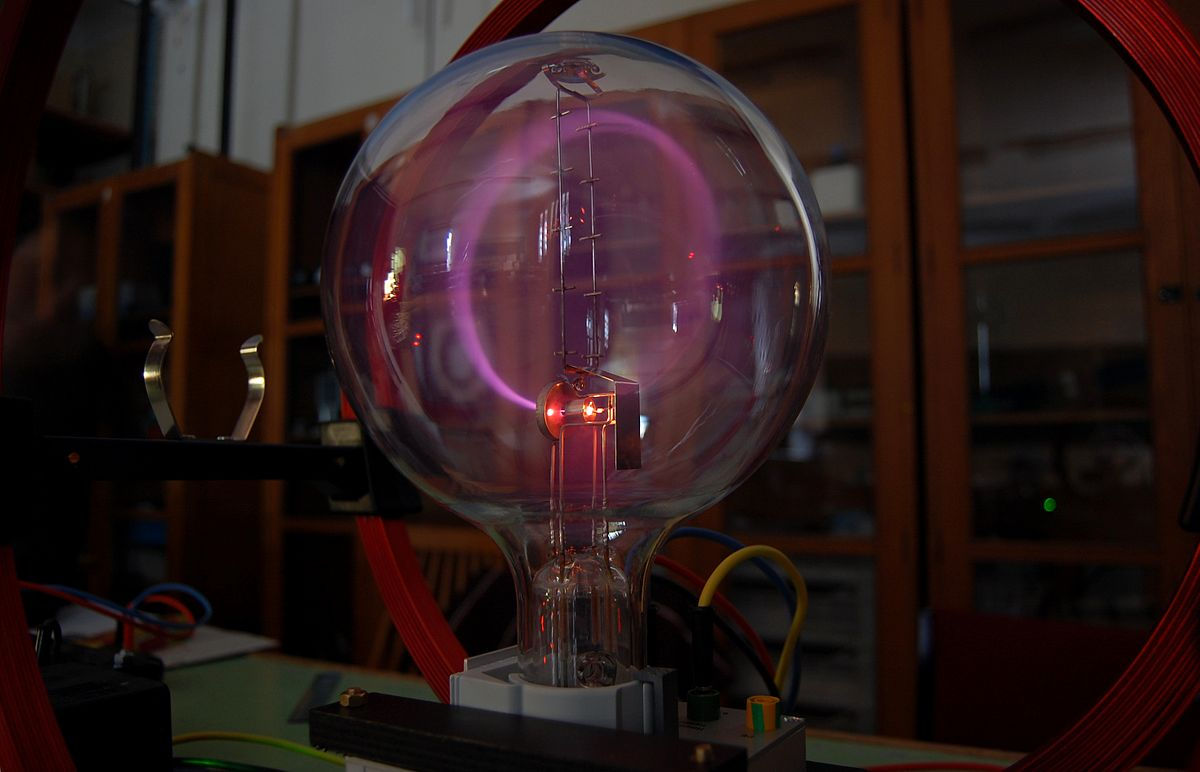
\includegraphics[width=0.7\textwidth]{Fadenstrahlrohr}
	\caption{Ein Fadenstrahlrohr}
	\label{fig:Fadenstrahlrohr}
\end{figure}

Ein Fadenstrahlrohr besteht aus einem Glaskolben in dem sich ein Gas befindet, welches beim Kontakt mit Elektronen zum Leuchten angeregt wird. Siehe Abbildung \ref{fig:Fadenstrahlrohr}\footnote{„Cyclotron motion wider view“ von Marcin Białek - Eigenes Werk. Lizenziert unter GFDL über Wikimedia Commons - \url{https://commons.wikimedia.org/wiki/File:Cyclotron\_motion\_wider\_view.jpg}}

Im Inneren befindet sich eine Elektronenkanone, die beschleunigte Elektronen absondert (Siehe: \referenz{sec:BraunscheRoehre}). Durch ein \emph{Helmholzspulenpaar} (2 kurze Spulen mit großem Radius) die parallel zur Richtung der beschleunigten Elektronen stehen, wird ein homogenes Magnetfeld erreicht, welches senkrecht auf der Elektronenrichtung steht.

\subsection{Beobachtung}

Die Elektronen beschreiben eine Kreisbahn, was am leuchtenden Gas zu sehen ist. Damit ist die Existenz einer Kraft auf bewegte, geladene Teilchen im Magnetfeld illustriert.

\subsection{Mathematisierung}

Wenn die Geschwindigkeit der Elektronen bekannt, bzw. errechnet wurde, kann über den Radius, welcher auch gemessen werden kann, die spezifische Elektronenladung bestimmt werden. Der Ansatz ist das Gleichsetzten der allgemeinen Zentripetalkraft $F_{Zp} = m \cdot \frac{v^2}{r}$, also die Kraft, die aufgewendet werden muss, um ein Elektron auf der Bahn zu halten, mit der Lorentzkraft  $F_{Lr} = q \cdot B \cdot v$, welche ja genau diese Bahn bewirkt:

\begin{align}
\begin{split}
	F_{Zp} &= F_{Lr} \\
	m_e \cdot \frac{v^2}{r} &= q_e \cdot B \cdot v \\
	\frac{q_e}{m_e} &=\frac{v}{B \cdot r}
\end{split}
\end{align}

\noindent Da es 2 Variablen in der Gleichung gibt ($m_e$ und $q_e$), kann man mit diesem Versuch nur auf das \emph{Verhältnis} der Ladung und Masse schließen, die \glqq spezifische Elektronenmasse\grqq .

Über den Millikanversuch (siehe: \referenz{sec:Millikan}) konnte jedoch die Elektronenladung $q_e$ direkt bestimmt werden, sodass durch den Versuch mit dem Fadenstrahlrohr die Masse bestimmt werden konnte:

\begin{align}
\begin{split}
	\frac{q_e}{m_e} &=\frac{v}{B \cdot r} \\
	m_e &=\frac{q_e \cdot B \cdot r}{v}
\end{split}
\end{align}





